
\chapter[Algorithmes séquentiels]{
Algorithmes séquentiels}
{
Avec ce chapitre, vous apprendrez à écrire un algorithme séquentiel pour
résoudre un problème informatique. C'est aussi
l'occasion de fixer la syntaxe du pseudo-code que nous
allons utiliser. Nous commençons dans ce chapitre avec les algorithmes
séquentiels qui sont de simples séquences de suites
d'instructions. Les structures alternatives et
répétitives seront vues dans les chapitres suivants. }

\begin{center}
 [Warning: Image ignored] % Unhandled or unsupported graphics:
%
\includegraphics[width=1.27cm,height=1.27cm]{log1-img/log1-img32}

\end{center}
\section{Introduction}
{
\textstylePolicepardfaut{Supposons que nous voulions rédiger une marche
à suivre détaillée qui explique comment additionner deux fractions. Une
possibilité de l’écrire en langage «~naturel~» serait la suivante :}}

\liststyleListii
\begin{itemize}
\item {\sffamily
\textstylePolicepardfaut{\textcolor{black}{Rechercher le dénominateur
commun des deux
fractions}}\textstylePolicepardfaut{\textcolor{black}{~}}\textstylePolicepardfaut{\textcolor{black}{;}}}
\item {\sffamily
\textstylePolicepardfaut{\textcolor{black}{Mettre chaque fraction au
même
dénominateur}}\textstylePolicepardfaut{\textcolor{black}{~}}\textstylePolicepardfaut{\textcolor{black}{;}}}
\item {\sffamily
\textstylePolicepardfaut{\textcolor{black}{Additionner les numérateurs
des deux fractions, }}}
\item {\sffamily
\textstylePolicepardfaut{\textcolor{black}{\ \ ce qui donne le
numérateur de la somme}}\textstylePolicepardfaut{\textcolor{black}{
;}}}
\item {\sffamily
\textstylePolicepardfaut{\textcolor{black}{Simplifier la fraction
obtenue.}}}
\end{itemize}
{
\textstylePolicepardfaut{Cet algorithme, bien que résultant d’un effort
d’explicitation, est encore très imprécis et risque fort de ne pas
faciliter l’effort de programmation qui en suivrait. N’oublions pas
qu’un ordinateur n’est qu’une machine dépourvue de toute intelligence
et incapable de comprendre les sous-entendus qu’un être humain pourrait
comprendre !}}

{
\textstylePolicepardfaut{De plus, les notions de dénominateur commun et
de simplification de fraction, bien qu'élémentaires
pour le cerveau, ne sont pas immédiates d'un point de
vue algorithmique. Un algorithme proche d'un langage
de programmation ne devrait mentionner que les opérations élémentaires
de calcul telles que +, –, *, /.}}

{
\textstylePolicepardfaut{Ceci dit, afin d’être plus proche d’un
programme écrit dans un langage compréhensible par l’ordinateur,
l’algorithme ci-dessus pourrait s’écrire :}}

\liststyleListii
\begin{itemize}
\item {\sffamily
\textstylePolicepardfaut{\textcolor{black}{Prendre connaissance du
premier numérateur et du premier dénominateur ;}}}
\item {\sffamily
\textstylePolicepardfaut{\textcolor{black}{Prendre connaissance du
second numérateur et du second dénominateur ;}}}
\item {\sffamily
\textstylePolicepardfaut{\textcolor{black}{Multiplier les deux
dénominateurs pour obtenir le dénominateur commun ;}}}
\item {\sffamily
\textstylePolicepardfaut{\textcolor{black}{Multiplier le premier
numérateur par le second dénominateur 
\ \ et le second numérateur par le premier dénominateur ;}}}
\item {\sffamily
\textstylePolicepardfaut{\textcolor{black}{Additionner ces deux produits
pour obtenir le numérateur du résultat ;}}}
\item {\sffamily
\textstylePolicepardfaut{\textcolor{black}{Communiquer ce résultat ainsi
que le dénominateur commun.}}}
\end{itemize}
{
\textstylePolicepardfaut{Notons encore que cet algorithme n’est pas le
plus efficace pour ce type de }\textstylePolicepardfaut{problème. Il
vaudrait mieux utiliser le PPCM (}\textstylePolicepardfaut{\textit{Plus
Petit Commun Multiple}}\textstylePolicepardfaut{) pour le
}\textstylePolicepardfaut{calcul du dénominateur commun, mais la façon
de calculer ce dernier serait très fastidieuse à rédiger en langage
«~naturel~». }}

{
\textstylePolicepardfaut{On comprend bien au travers de cet exemple que
le français n’est pas adapté à la description de problèmes au contenu
mathématique ou scientifique. Le langage naturel est, en effet, un mode
de représentation trop riche des algorithmes. Il faut comprendre par
«~riche~», la présence de synonymes, de nombreux mots aux
significations proches et voisines. L’utiliser amènerait probablement à
une perte de temps (donc d’argent), et à des risques d’erreurs dans la
conception des programmes. Il convient dès lors d’élaborer des méthodes
de représentation plus rigoureuses (donc moins riches) mais nécessitant
un effort moindre de programmation.}}

{
\textstylePolicepardfaut{Ceci dit, le français peut toujours être
utilisé dans la formalisation d’une première approche de la résolution
d’un problème devant être traduit ensuite en algorithme puis en
programme.}}

\section[Le pseudo{}-code]{\bfseries Le pseudo-code}
{
Les inconvénients de l’utilisation du français dans la représentation
des algorithmes sont dus à la trop grande richesse de ce langage en
comparaison à la pauvreté (mais aussi la rigueur) du langage compris
par la machine. De plus, la lourdeur et la longueur des phrases
risquent de rendre pénible la relecture et le travail d’élaboration des
algorithmes. La solution consiste à édulcorer le langage naturel, d’une
part en remplaçant les noms parfois fastidieux des objets sur lesquels
portent des opérations par des mots (noms de variables) plus courts,
d’autre part, en remplaçant les opérations elles-mêmes par des
opérateurs symboliques suffisamment explicites. De plus, des structures
types remplaceront les multiples possibilités linguistiques signifiant
la même chose.}

{
Le \textbf{pseudo-code} ou \textit{Langage de Description des
Algorithmes} (LDA en abrégé) est un langage formel et symbolique
utilisant :}

\begin{center}
 [Warning: Image ignored] % Unhandled or unsupported graphics:
%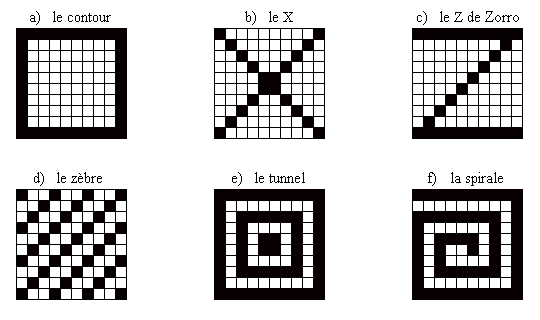
\includegraphics[width=1.129cm,height=1.282cm]{log1-img/log1-img33}

\end{center}
\liststyleListv
\begin{itemize}
\item {
des \textbf{noms symboliques} destinés à représenter les objets sur
lesquels s’effectuent des actions ;}
\item {
des \textbf{opérateurs symboliques} ou des mots-clés traduisant les
opérations primitives exécutables par un exécutant donné ;}
\item {
des \textbf{structures de contrôle} types.}
\end{itemize}
{
Ce langage repose sur des conventions d’écriture. Il est destiné à
servir de vecteur de la compréhension permettant par exemple une
relecture faite par l’élaborateur de l’algorithme lui-même ou faite par
autrui et facilitant le travail de programmation.}

{
C’est de cette dernière exigence que nait la polémique consistant à
savoir jusqu’à quel niveau de détail il convient d’aller dans la
représentation d’un algorithme ! Nous dirons, pour notre part, qu’il ne
doit jamais être aussi détaillé que le programme lui-même, celui-ci
étant, par essence, la description ultime. Point n’est besoin de donner
deux descriptions quasi identiques d’un algorithme, l’une dans un
langage \textit{pseudo-codé}, l’autre exprimée dans un langage de
programmation.}

{
Nous dirons qu’un algorithme \textit{idéal}, appelé \textbf{algorithme
général}, exprimé en pseudo-code, devrait se situer à mi-chemin entre
la démarche globale exprimée dans un langage naturel (langue française)
ou structuré (ordinogramme) et l’algorithme ultime, c’est-à-dire le
\textbf{programme}, exprimé en langage de programmation.}

{
On pourrait d’ailleurs concevoir la possibilité d’établir d’autres
\textbf{algorithmes plus }\textbf{détaillés} se situant entre
l’algorithme général et le programme et qui tiendraient compte de
certaines particularités du langage de programmation dans lequel ils
sont destinés à être traduits.}

{
Enfin, et ce n’est pas la chose la moins importante, la définition d’un
pseudo-code doit être telle qu’il puisse \textbf{faciliter
l’apprentissage d’une logique de programmation} par des personnes
désireuses de faire de l’informatique un métier. Dans cette optique, il
est inutile de les embarrasser de contraintes syntaxiques ou autres qui
risquent de les éloigner du but poursuivi.}

{
En conclusion, à partir du moment où des conventions sont prises dans un
contexte bien déterminé (un service informatique d’une entreprise, un
groupe scolaire,...), il convient que \textbf{tous }respectent ces
conventions. Ce sera à chacun de juger jusqu’où il ne faut pas aller
trop loin dans la liberté d’écriture.}

\section[Variables et types]{\bfseries Variables et types}
{
Nous savons que les opérations que l’ordinateur devra exécuter portent
sur des éléments qui sont les \textbf{données} du problème. Lorsqu’on
attribue un \textbf{nom} et un \textbf{type} à ces données, on parle
alors de \textbf{variables}. Dans un algorithme, une variable conserve
toujours son nom et son type, mais peut changer de \textbf{valeur}.}

{
Le \textbf{nom }d’une variable permet de la caractériser et de la
reconnaitre. Ainsi, dans l’exemple donné ci-dessus, nous pourrions
donner le nom \textit{num1} au \textit{premier numérateur} et
\textit{num2} au \textit{second numérateur}, ce qui permet déjà de
nommer les objets de l’algorithme de façon tout aussi reconnaissable
mais plus courte et donc plus commode. Quant au \textbf{type} d’une
variable, il décrit la nature de son contenu. }

{\sffamily\bfseries\upshape
Les types autorisés}

{
Dans un premier temps, les seuls \textbf{types} utilisés sont les
suivants :}

\begin{center}
 [Warning: Image ignored] % Unhandled or unsupported graphics:
%\includegraphics[width=1.129cm,height=1.282cm]{log1-img/log1-img34}

\end{center}
\begin{center}
\tablehead{}
\begin{supertabular}{m{1.8109999cm}|m{11.918cm}}
\raggedleft  \textstyleMotCl{entier} &
 pour les nombres entiers\\
\raggedleft  \textstyleMotCl{réel} &
 pour les nombres réels\\
\raggedleft  \textstyleMotCl{caractère} &
 pour les différentes lettres et caractères (par
exemple ceux qui apparaissent sur un clavier : ‘a’, ‘1’, ‘\#’, etc…)\\
\raggedleft  \textstyleMotCl{chaine} &
{ pour les variables contenant plusieurs
caractères ou aucun}

 (la chaine vide)\\
\raggedleft  \textstyleMotCl{booléen} &
 les variables de ce type ne peuvent valoir que
\textbf{vrai} ou \textbf{faux}\\
\end{supertabular}
\end{center}
{
On veillera au cours de logique à ne pas utiliser les valeurs 0 et 1
pour les variables booléennes, même si leur emploi est correct dans
beaucoup de langages de programmation.}

{\sffamily\bfseries\scshape
Exercice : Une date}

\begin{center}
 [Warning: Image ignored] % Unhandled or unsupported graphics:
%
\includegraphics[width=1.282cm,height=1.282cm]{log1-img/log1-img35}

\end{center}
{
Quel(s) type(s) de données utiliseriez-vous pour représenter une date du
calendrier ? }

{\sffamily\bfseries\scshape
Exercice : Un moment}

\begin{center}
 [Warning: Image ignored] % Unhandled or unsupported graphics:
%
\includegraphics[width=1.282cm,height=1.282cm]{log1-img/log1-img36}

\end{center}
{
Quel(s) type(s) de données utiliseriez-vous pour représenter un moment
dans la journée ? }

{\sffamily\bfseries\upshape
Déclaration de variables}

{
La déclaration d’une variable est l’instruction qui définit son nom et
son type. On pourrait écrire :}

{\sffamily
num1 et num2 seront les noms de deux objets destinés à recevoir les}

{\sffamily
numérateurs des fractions, c’est-à-dire des nombres à valeurs entières.}

{
\textcolor{black}{Mais, bien entendu, cette formulation, trop proche du
langage parlé, }serait trop floue et trop longue. Dès lors, nous
abrégerons par :}

{\sffamily
num1, num2 : entiers}

{
L’ensemble des instructions de la forme}

{\sffamily
variable1, variable2, … : type}

\begin{center}
 [Warning: Image ignored] % Unhandled or unsupported graphics:
%
\includegraphics[width=1.129cm,height=1.282cm]{log1-img/log1-img37}

\end{center}
{
forme la partie d’un algorithme nommée \textbf{déclaration des
variables}. La déclaration des informations apparaitra toujours en
début d’algorithme, ou dans un bloc annexe appelé \textbf{dictionnaire
des variables} ou encore \textbf{dictionnaire des données}.}

{
Par exemple, pour l’algorithme des fractions, la déclaration des
informations pourrait être la suivante :}

{\sffamily
num1, den1, num2, den2, numRes, denRes : entiers}

{
avec la signification suivante :}

{
\ \ \textstyleCodeInsr{\textcolor{black}{num1 }}\textcolor{black}{(
}\textstyleCodeInsr{\textcolor{black}{num2}}\textcolor{black}{
)}\textcolor{black}{\ \ \ \ pour numérateur de la première (seconde)
fraction ;}}

{
\textcolor{black}{\ \ }\textstyleCodeInsr{\textcolor{black}{den1}}\textcolor{black}{
( }\textstyleCodeInsr{\textcolor{black}{den2}}\textcolor{black}{
)}\textcolor{black}{\ \ \ \ pour dénominateur de la première (seconde)
fraction ;}}

{
\textcolor{black}{\ \ }\textstyleCodeInsr{\textcolor{black}{numRes}}\textcolor{black}{
( }\textstyleCodeInsr{\textcolor{black}{denRes
}}\textcolor{black}{)}\textcolor{black}{\ \ pour numérateur
(dénominateur) du résultat.}}

{
Attention, lors de la déclaration d’une variable, celle-ci n’a pas de
valeur ! Nous verrons plus loin que c’est l’instruction
d’\textbf{affectation} qui va servir à donner un contenu aux variables
déclarées. En logique, nous n’envisageons pas d’\textit{affectation par
défaut} consistant à donner une valeur initiale de façon automatique
aux variables déclarées (par exemple 0 pour les variables numériques,
comme c’est le cas dans certains langages informatiques).}

\begin{center}
 [Warning: Image ignored] % Unhandled or unsupported graphics:
%
\includegraphics[width=1.323cm,height=1.323cm]{log1-img/log1-img38}

\end{center}
{\sffamily\bfseries
Comment nommer correctement une variable ?}

{
Le but est de trouver un nom qui soit suffisamment court tout en restant
explicite (ainsi \textstyleCodeInsr{num1} est plus approprié pour
désigner le \textit{premier numérateur }que \textstyleCodeInsr{zozo1},
\textstyleCodeInsr{tintin}, \textstyleCodeInsr{bidule,
premierNumérateur}) et qui ne prête pas à confusion (par exemple ne pas
utiliser un des mots réservés du pseudo-code comme
\textstyleMotCl{\textsf{lire}}, \textstyleMotCl{\textsf{écrire}},
\textstyleMotCl{\textsf{pour}}…). Il faut aussi tenir compte que les
langages de programmation imposent certaines limitations (parfois
différentes d'un langage à l'autre)
ce qui peut nécessiter une modification du nom lors de la traduction.}

{
Voici quelques règles et limitations traditionnelles dans les langages
de programmation: }

\liststyleListv
\begin{itemize}
\item {
Un nom de variable est généralement une suite de caractères
alphanumériques d’un seul tenant (pas de caractères blancs) et ne
commençant jamais par un chiffre. Ainsi \textstyleCodeInsr{x1} est
correct mais non \textstyleCodeInsr{1x}. }
\item {
Pour donner un nom composé à une variable, on peut utiliser le «~tiret
bas~» ou \textit{underscore} (par ex. premier\_numérateur) mais on
déconseille d’utiliser le signe «~–~» qui est plutôt réservé à la
soustraction. Ainsi, dans la plupart des langages,
\textstyleCodeInsr{premier-numérateur} serait interprété comme la
soustraction des variables \textstyleCodeInsr{premier} et
\textstyleCodeInsr{numérateur}. (Signalons que le tiret 
\textcolor{black}{«~–~»} est autorisé en Cobol, où il récupère son rôle
arithmétique s’il est précédé et suivi d’au moins un blanc). }
\item {
Une alternative à l’utilisation du tiret bas pour l’écriture de noms de
variables composés est la notation «~chameau~» (\textit{camelCase} en
anglais), qui consiste à mettre une majuscule au début des mots
(généralement à partir du deuxième), par exemple
\textstyleCodeInsr{premierNombre} ou
\textstyleCodeInsr{dateNaissance}.}
\item {
Les indices et exposants sont proscrits (par ex.
\textstyleCodeInsr{x}\textstyleCodeInsr{\textsubscript{1}},
\textstyleCodeInsr{z}\textstyleCodeInsr{\textsubscript{6}} ou
\textstyleCodeInsr{m²)} }
\item {
Les mots clés du langage sont interdits (par exemple
\textstyleMotCl{for}, \textstyleMotCl{if}, \textstyleMotCl{while }pour
Java et Cobol).}
\item {
Certains langages n’autorisent pas les caractères accentués (tels que
\textit{à, ç, ê, ø,} etc.) ou les lettres des alphabets non latins
(tels que ${\Delta}$ ou
\textsf{[635?][635?]}) mais d’autres oui ; certains font la distinction
entre les minuscules et majuscules, d’autres non. En logique, nous
admettons dans noms de variables les caractères accentués du français,
par ex. : durée, intérêts, etc. }
\end{itemize}
{
Il est impossible de décrire ici toutes les particularités des
différents langages, le programmeur se reportera aux règles spécifiques
du langage qu’il sera amené à utiliser.}

{\sffamily\bfseries\scshape
Exercice : Déclarer une date}

\begin{center}
 [Warning: Image ignored] % Unhandled or unsupported graphics:
%
\includegraphics[width=1.282cm,height=1.282cm]{log1-img/log1-img39}

\end{center}
{
Déclarer le(s) variable(s) permettant de représenter la date
d'anniversaire de quelqu'un.}

{\sffamily\bfseries\scshape
Exercice : Déclarer un rendez-vous}

\begin{center}
 [Warning: Image ignored] % Unhandled or unsupported graphics:
%\includegraphics[width=1.282cm,height=1.282cm]{log1-img/log1-img40}

\end{center}
{
Déclarer le(s) variable(s) permettant de représenter
l'heure de début, l'heure de fin et
l'objet d 'un rendez-vous.}

\section{Opérateurs et expressions}
{
Les opérateurs agissent sur les variables et les constantes pour former
des \textbf{expressions}. Une expression est donc une combinaison
\textbf{cohérente} de variables, de constantes et d’opérateurs,
éventuellement accompagnés de parenthèses.}

{\sffamily\bfseries\upshape
Opérateurs arithmétiques élémentaires}

{
Ce sont les opérateurs binaires bien connus : }

{
\textstyleCodeInsr{+}\ \ \ \ addition}

\begin{center}
 [Warning: Image ignored] % Unhandled or unsupported graphics:
%
\includegraphics[width=1.129cm,height=1.282cm]{log1-img/log1-img41}

\end{center}
{
\textstyleCodeInsr{–}\ \ \ \ soustraction}

{
\textstyleCodeInsr{*}\ \ \ \ multiplication}

{
\ \ \textstyleCodeInsr{/}\ \ \ \ \textcolor{black}{division réelle}}

{
Ils agissent sur des variables ou expressions à valeurs entières ou
réelles. Plusieurs opérateurs peuvent être utilisés pour former des
expressions plus ou moins complexes, en tenant compte des règles de
calcul habituelles, notamment la priorité de la multiplication et de la
division sur l’addition et la soustraction. Il est aussi permis
d’utiliser des parenthèses, par exemple \textstyleCodeInsr{a – (b + c *
d)/x}. Tout emploi de la division devra être accompagné d’une réflexion
sur la valeur du dénominateur, une division par 0 entrainant toujours
l’arrêt d’un algorithme.}

{\sffamily\bfseries
DIV et MOD}

{
Ce sont deux opérateurs très importants qui ne peuvent s’utiliser
qu’avec des variables entières :}

{
\textstyleCodeInsr{DIV} \ \ \ \ division entière}

\begin{center}
 [Warning: Image ignored] % Unhandled or unsupported graphics:
%
\includegraphics[width=1.129cm,height=1.282cm]{log1-img/log1-img42}

\end{center}
{
\textstyleCodeInsr{MOD} \ \ \ \ reste de la division entière}

{
Par exemple, \textstyleCodeInsr{47 DIV 7} donne 6 tandis que
\textstyleCodeInsr{47 MOD 7} donne \textstyleCodeInsr{5}.}

{\sffamily\bfseries\upshape
Fonctions mathématiques complexes}

{
L’élévation à la puissance sera notée \textstyleCodeInsr{**} ou
\textstyleCodeInsr{\^{}} . Pour la racine carrée d’une variable x nous
écrirons  $\sqrt{x}$ \textit{.} Attention, pour ce dernier, de veiller
à ne l’utiliser qu’avec un radicant positif !}

{
 $\frac{-b+\sqrt{b^{2}-4\ast a\ast c}}{2\ast a}$ \textbf{Exemple} : 
$(-b+\sqrt{(b\ast \ast 2-4\ast a\ast c)})/(2\ast a)$ }

{
Mais on peut aussi accepter la notation mathématique usuelle }

{
Pourquoi ne pas avoir écrit «~\textstyleCodeInsr{4ac}~» et
«~\textstyleCodeInsr{2a}~» ?}

\begin{center}
 [Warning: Image ignored] % Unhandled or unsupported graphics:
%
\includegraphics[width=1.244cm,height=1.296cm]{log1-img/log1-img43}

\end{center}
{
Si nécessaire, on se permettra d'utiliser les autres
fonctions mathématiques sous leur forme la plus courante dans la
plupart des langages de programmation (exemples :
\textstyleCodeInsr{sin(x), tan(x), log(2*x), exp(a-b)}, ...)}

{\sffamily\bfseries
Opérateurs logiques}

{
Ils agissent sur des expressions booléennes (variables ou expressions à
valeurs booléennes) pour donner un résultat du même type.}

{
\ \ \textstyleCodeInsr{NON}\ \ \ \ négation}

\begin{center}
 [Warning: Image ignored] % Unhandled or unsupported graphics:
%
\includegraphics[width=1.129cm,height=1.282cm]{log1-img/log1-img44}

\end{center}
{
\ \ \textstyleCodeInsr{ET} \ \ \ \ conjonction logique}

{
\ \ \textstyleCodeInsr{OU} \ \ \ \ disjonction logique}

{
Pour rappel, \textstyleCodeInsr{cond1 ET cond2} n’est vrai que lorsque
les deux conditions sont vraies. \textstyleCodeInsr{cond1 OU cond2} est
toujours vrai, sauf quand les deux conditions sont fausses.}

{
Veillez à mettre des parenthèses dans le cas de combinaisons de ET et de
OU : \textstyleCodeInsr{(cond1 ET cond2) OU cond3} étant différent de
\textstyleCodeInsr{cond1 ET (cond2 OU cond3).} En cas
d'oubli de parenthèses, il faudra se rappeler que
\textstyleCodeInsr{ET} est prioritaire sur le \textstyleCodeInsr{OU}. }

{\sffamily\bfseries\upshape
Évaluation complète et court-circuitée}

{
On définit deux modes d’évaluation des opérateurs \textstyleCodeInsr{ET}
et \textstyleCodeInsr{OU} :}

\liststyleListv
\begin{itemize}
\item {
l’évaluation \textit{complète} : pour connaitre la valeur de
\textstyleCodeInsr{cond1 ET cond2} (respectivement
\textstyleCodeInsr{cond1 OU cond2}), les deux conditions sont chacune
évaluées, après quoi on évalue la valeur de vérité de l’ensemble de
l'expression.}
\item {
l’évaluation \textit{court-circuitée} : dans un premier temps, seule la
première condition est testée. Dans le cas du \textstyleCodeInsr{ET},
si \textstyleCodeInsr{cond1} s’avère faux, il est inutile d’évaluer
\textstyleCodeInsr{cond2} puisque le résultat sera faux de toute façon
; l’évaluation de \textstyleCodeInsr{cond2} et de l’ensemble de la
conjonction ne se fera que si \textstyleCodeInsr{cond1} est vrai. De
même, dans le cas du \textstyleCodeInsr{OU}, si
\textstyleCodeInsr{cond1} s’avère vrai, il est inutile d’évaluer
\textstyleCodeInsr{cond2} puisque le résultat sera vrai de toute façon
; l’évaluation de \textstyleCodeInsr{cond2} et de l’ensemble de la
disjonction ne se fera que si \textstyleCodeInsr{cond1} est faux. }
\end{itemize}
{
Dans le cadre de ce cours, nous opterons pour la deuxième définition.
Montrons sur un exemple l’avantage de cette interprétation. Considérons
l’expression 
\textstyleCodeInsr{n }\textstyleCodeInsr{${\neq}$}\textstyleCodeInsr{ 0
ET s/n {\textgreater} 10}. Si on teste sa valeur de vérité avec une
valeur de \textstyleCodeInsr{n} non nulle, la première condition est
vraie et le résultat de la conjonction dépendra de la valeur de la
deuxième condition. Supposons à présent que \textstyleCodeInsr{n} soit
nul. L’évaluation court-circuitée donne le résultat \textbf{faux}
immédiatement après test de la première condition sans évaluer la
seconde, tandis que l’évaluation complète entrainerait un arrêt de
l’algorithme pour cause de division par 0 ! }

{
Noter que l’évaluation court-circuitée a pour conséquence la
non-commutativité du \textstyleCodeInsr{ET} et du
\textstyleCodeInsr{OU~}: \textstyleCodeInsr{cond1 ET cond2} n’est donc
pas équivalent à \textstyleCodeInsr{cond2 ET cond1}, puisque l’ordre
des évaluations des deux conditions entre en jeu.~Nous conseillons
cependant de limiter les cas d’utilisation de l’évaluation
court-circuitée et d'opter pour des expressions dont
l’évaluation serait similaire dans les deux cas. La justification
d’utiliser l’évaluation court-circuitée apparaitra dans plusieurs
exemples tout au long du cours. }

{\sffamily\bfseries
Opérateurs de comparaison}

{
Ces opérateurs agissent généralement sur des variables numériques ou des
chaines et donnent un résultat booléen. }

{
\textstyleCodeInsr{{\textless}} \ \ \ \ (strictement) plus petit que}

\begin{center}
 [Warning: Image ignored] % Unhandled or unsupported graphics:
%\includegraphics[width=1.129cm,height=1.282cm]{log1-img/log1-img45}

\end{center}
{
\textstyleCodeInsr{{\textgreater}} \ \ \ \ (strictement) plus grand que}

{
\textstyleCodeInsr{=} \ \ \ \ égal}

{
\textstyleCodeInsr{{\textless}{\textgreater}} ou
\textstyleCodeInsr{${\neq}$} \ \ différent de}

{
\textstyleCodeInsr{${\leq}$}\ \ \ \ plus petit ou égal}

{
\textstyleCodeInsr{${\geq}$}\ \ \ \ plus grand ou égal}

{
Pour les chaines, c'est l’ordre alphabétique qui
détermine le résultat (par exemple
\textstyleCodeInsr{{\textquotedbl}milou{\textquotedbl} {\textless}
{\textquotedbl}tintin{\textquotedbl}} est \textbf{vrai} de même que
\textstyleCodeInsr{{\textquotedbl}assembleur{\textquotedbl}
}\textstyleCodeInsr{${\leq}$}\textstyleCodeInsr{
{\textquotedbl}java{\textquotedbl}})}

\section{L’affectation d’une valeur à une variable}
{
Cette opération est probablement l’opération la plus importante. En
effet, une variable ne prend son sens réel que si elle reçoit à un
moment donné une valeur. Il y a deux moyens de donner une valeur à une
variable.}

{\sffamily\bfseries
Affectation externe }

{
On parle d’\textbf{affectation externe} lorsque la valeur à affecter à
une variable est donnée par l’utilisateur qui la communique à
l’exécutant quand celui-ci le lui demande : cette valeur est donc
\textit{externe} à la procédure \ (l’ordinateur ne peut la deviner
lui-même !)}

{
L’affectation externe est donc la primitive qui permet de recevoir de
l’utilisateur, au moment où l'algorithme se déroule,
une ou plusieurs valeur(s) et de les affecter à des variables en
mémoire. Nous noterons :}

{\sffamily
\textstyleMotCl{lire} liste\_de\_variables\_à\_lire}

\begin{center}
 [Warning: Image ignored] % Unhandled or unsupported graphics:
%
\includegraphics[width=1.129cm,height=1.282cm]{log1-img/log1-img46}

\end{center}
{\bfseries
Exemples}

{\sffamily
\textstyleMotCl{lire} nombre1, nombre2}

{\sffamily
\textstyleMotCl{lire} num1, den1, num2, den2}

{
{L’exécution de }cette instruction provoque une
pause dans le déroulement de l’algorithme : l’exécutant demande alors à
l’utilisateur les valeurs des variables à lire. Ces valeurs viennent
donc de l’\textit{extérieur~}; une fois introduites dans le système,
elles sont affectées aux variables concernées et l’algorithme peut
reprendre son cours. Par \textit{extérieur} nous entendons ici tout
support d’introduction des données extérieur à la mémoire du programme.
Les possibilités sont nombreuses : citons par exemple l’encodage de
données au clavier, un clic de souris, le toucher d'un
écran tactile, des données provenant d’un fichier, etc.}

{\sffamily\bfseries
Affectation interne }

{
On parle d’affectation interne lorsque la valeur d’une variable est
«~calculée~» par l’exécutant de l’algorithme lui-même à partir de
données qu’il connait déjà :}

{\sffamily
\textbf{nomVariable }{\textbf{←}}\textbf{
expression}}

\begin{center}
 [Warning: Image ignored] % Unhandled or unsupported graphics:
%
\includegraphics[width=1.129cm,height=1.282cm]{log1-img/log1-img47}

\end{center}
{
Rappelons qu’une \textbf{expression} est une combinaison de variables et
d’opérateurs. }

{\bfseries
Exemples}

{\sffamily
somme {\textbf{←}} nombre1 + nombre2}

{\sffamily
denRes {\textbf{←}} den1 * den2}

{\sffamily
cpt {\textbf{←}} cpt + 1}

{\sffamily
delta {\textbf{←}} b**2 – 4*a*c}

{\sffamily
test {\textbf{←}} a {\textless} b \ \ \ \ //
pour une variable logique}

{\bfseries
Remarques}

\liststyleListv
\begin{itemize}
\item {
Il est de règle que le résultat de l’expression à droite du signe
d’affectation ({\textsf{\textbf{←}}}) soit de
même type que la variable à sa gauche. On tolère certaines exceptions
:}
\item {
\textstyleCodeInsr{entier
}\textstyleCodeInsr{{\textbf{←}}}\textstyleCodeInsr{
réel} : \ dans ce cas le contenu de la variable sera la valeur tronquée
de l’expression réelle. Par exemple si «~\textstyleCodeInsr{nb~»} est
une variable de type entier, son contenu après l’instruction
«~\textstyleCodeInsr{nb
}\textstyleCodeInsr{{\textbf{←}}}\textstyleCodeInsr{
15/4~»} sera 3}
\item {
\textstyleCodeInsr{réel
}\textstyleCodeInsr{{\textbf{←}}}\textstyleCodeInsr{
entier} : \ ici, il n'y a évidemment pas de perte de
valeur.}
\item {
\textstyleCodeInsr{chaine
}\textstyleCodeInsr{{\textbf{←}}}\textstyleCodeInsr{
caractère;} le contraire n'est évidemment pas
accepté.}
\item {
Seules les variables déclarées peuvent être affectées, que ce soit par
l’affectation externe ou interne!}
\item {
On veillera à ne pas mélanger la déclaration d’une variable et son
affectation interne dans une même ligne de code, donc pas
d’instructions hybrides du genre \textsf{x}\textstyleCodeInsr{
}\textstyleCodeInsr{{\textbf{←}}}\textstyleCodeInsr{
2 : entier}\ \ // incorrect !}
\item {
Pour l’affectation interne, toutes les variables apparaissant dans
\textstyleCodeInsr{expression} doivent avoir été affectées
préalablement. Le contraire provoquerait un arrêt de l’algorithme.}
\end{itemize}
\section{Communication des résultats}
{
L’instruction de communication des résultats consiste à donner à
l’extérieur (donc à l’utilisateur) la valeur d’un résultat de
l’exécution de l’algorithme. Nous écrirons :}

{\sffamily
\textstyleMotCl{écrire} expression ou liste de variables}

\begin{center}
 [Warning: Image ignored] % Unhandled or unsupported graphics:
%
\includegraphics[width=1.129cm,height=1.282cm]{log1-img/log1-img48}

\end{center}
{
qui signifie que la valeur d’une expression (ou celles des différentes
variables mentionnées) sera fournie à l’utilisateur (par exemple par un
affichage à l’écran ou par impression sur listing via l’imprimante,
etc…).}


\bigskip

{\bfseries
Remarques}

\liststyleListv
\begin{itemize}
\item {
Ce ne serait pas une erreur fondamentale de remplacer
\textstyleCodeInsr{lire} par \textstyleCodeInsr{recevoir} ou
\textstyleCodeInsr{écrire} par \textstyleCodeInsr{afficher}. Il n’y a
évidemment pas de confusion possible à partir du moment où l’on sait
qu’il s’agit de primitives d’échange entre l’extérieur et l’ordinateur
exécutant la procédure, mais par principe, il est conseillé d’utiliser
une syntaxe commune et limitée à un petit nombre de mots clés. }
\item {
Comme pour l’affectation interne, on ne peut \textstyleCodeInsr{écrire}
que des expressions dont les variables ont été affectées préalablement.
}
\end{itemize}
\section{Structure générale d’un algorithme}
{
La traduction d’un algorithme en pseudo-code constituera le contenu d’un
\textstyleMotCl{module}. Un module contient donc la solution
algorithmique d’un problème donné (ou d’une de ses parties). Sa
structure générale sera la suivante :}

{\sffamily
\textstyleMotCl{module} nomDuModule()}

\begin{center}
 [Warning: Image ignored] % Unhandled or unsupported graphics:
%
\includegraphics[width=1.129cm,height=1.282cm]{log1-img/log1-img49}

\end{center}
{\sffamily
\ \ \textit{déclaration des variables et constantes utilisées dans le
module}}

{\sffamily\itshape
\ \ lecture des données}

{\sffamily\itshape
\ \ instructions utilisant les données lues}

{\sffamily\itshape
\ \ \ communication des résultats}

{\sffamily
\textstyleMotCl{fin} \textstyleMotCl{module}}


\bigskip

{\bfseries
Remarques}

\liststyleListv
\begin{itemize}
\item {
Le code d'un algorithme sera toujours compris entre la
première ligne ; appelée «~entête~» qui commence par le mot «~module~»
suivi du nom choisi pour l'algorithme ; et la ligne
finale «~fin module~». Le code compris entre l'entête
et la ligne finale sera toujours légèrement décalé vers la droite,
c'est un premier exemple
d'\textbf{indentation} indispensable pour la
lisibilité d'un programme, nous y reviendrons lors de
l'étude des structures alternatives et répétitives.}
\item {
Comme pour les variables, le nomDuModule devra être approprié au contenu
! Par exemple, sommeNombres, additionnerFractions plutôt que goPartez
!
Le rôle des parenthèses qui suivent le nom du module sera expliqué plus
tard.}
\item {
Il va de soi que toutes les parties de cette structure générale ne
seront pas toujours nécessaires : certains algorithmes ne nécessiteront
pas de lecture de données, d'autres ne devront pas
communiquer des résultats,...}
\item {
Pour la lisibilité, on veillera toujours à ce que le texte d’un module
tienne sur une seule page.}
\end{itemize}
{
À titre d’exemple, récrivons l’algorithme d’addition de fractions décrit
en début de chapitre :}

{\sffamily
\textstyleMotCl{module} additionnerFractions()}

{\sffamily
\ \ num1, den1, num2, den2, numRes, denRes : entiers}

{\sffamily
\textstyleMotCl{\ \ lire} num1, den1, num2, den2}

{\sffamily
{\ \ denRes
}{\textbf{←}}{ den1 *
den2}}

{\sffamily
{\ \ numRes
}{\textbf{←}}{
num1*den2 + num2*den1}}

{\sffamily
\textstyleMotCl{\ \ écrire} numRes, {\textquotedbl}~/~{\textquotedbl},
denRes}

{\sffamily
\textstyleMotCl{fin} \textstyleMotCl{module}}


\bigskip

\section[Commenter un algorithme]{\bfseries Commenter un
algorithme}
{
On n’insistera jamais assez sur la nécessité de \textbf{documenter} un
algorithme en y insérant des \textbf{commentaires} judicieux, clairs et
suffisants ! Un commentaire est un texte placé dans
l'algorithme et destiné à faciliter au maximum la
compréhension d’un algorithme par le lecteur (parfois une autre
personne, mais aussi souvent l'auteur qui se perd dans
son propre texte lorsqu'il y replonge après une
interruption). Ces commentaires (introduits par
«~\textstyleCodeInsr{//~» }) seront bien entendu ignorés par
l’exécutant de l’algorithme.}

{\sffamily
// ce module lit les contenus de 2 fractions et affiche leur somme}

{\sffamily
\textstyleMotCl{module} additionnerFractions()}


\bigskip

{\sffamily
\ \ num1, den1, num2, den2, numRes, denRes : entiers}


\bigskip

{\sffamily
\ \ \textstyleMotCl{lire} num1, den1, num2, den2}

{\sffamily
{\ \ denRes
}{\textbf{←}}{ den1 *
den2 \ \ \ \ \ \ \ \ \ \ \ \ \ \ \ \ \ \ // calcul du dénominateur}}

{\sffamily
{\ \ numRes
}{\textbf{←}}{
num1*den2 + num2*den1\ \ // calcul du numérateur}}

{\sffamily
\ \ \textstyleMotCl{écrire} numRes, {\textquotedbl}~/~{\textquotedbl},
denRes\ \  \ // la fraction n'est sans doute pas
simplifiée}


\bigskip

{\sffamily
\textstyleMotCl{fin} \textstyleMotCl{module}}

{
Noter qu’un excès de commentaires peut être aussi nuisible qu’un
trop-peu pour la compréhension d’un algorithme. Par exemple, un choix
judicieux de noms de variables peut s’avérer bien plus efficace que des
commentaires superflus. Ainsi, l’instruction}

{\sffamily
nouveauCapital {\textbf{←}} ancienCapital * (1 +
taux / 100)}

{
dépourvue de commentaires est bien préférable aux lignes suivantes :}

{\sffamily
c1 {\textbf{←}} c0 * (1 + t / 100) \ // calcul
du nouveau capital}

{\sffamily
\ \ \ \ \ \ // c1 est le nouveau capital, c0 est l’ancien capital, t est
le taux}

\section{Compléments de pseudo-code}
{
\textstyleMotCl{\textmd{Présentons quelques notions algorithmiques peu
utilisées en première mais qui vous seront peut-être utiles dans
l'un ou l'autre des exercices.}}}

{\sffamily\bfseries\upshape
Constantes}

{
Une \textbf{constante} est une information pour laquelle nom, type et
valeur sont figés. La liste des constantes utilisées dans un algorithme
apparaitra dans la section déclaration des variables sous la forme
suivante :}

{\sffamily
\textstyleMotCl{constante} PI = 3,14}

\begin{center}
 [Warning: Image ignored] % Unhandled or unsupported graphics:
%
\includegraphics[width=1.129cm,height=1.282cm]{log1-img/log1-img50}

\end{center}
{\sffamily
\textstyleMotCl{constante} ESI = {\textquotedbl}École Supérieure d’
Informatique{\textquotedbl}}

{
\textstyleMotCl{\textmd{Il est inutile de spécifier leur type, celui-ci
étant défini implicitement par la valeur de la constante.}}}

{\sffamily\bfseries\upshape
Énumération}

{
Parfois, une variable ne peut prendre qu'un ensemble
fixe et fini de valeurs. Par exemple une variable représentant une
saison ne peut prendre que quatre valeurs (HIVER, PRINTEMPS, ETE,
AUTOMNE). On va l'indiquer grâce à
l'énumération qui introduit un \textbf{nouveau type}
de donnée.}

{\sffamily
\textstyleMotCl{énumération} Saison \{ HIVER, PRINTEMPS, ETE, AUTOMNE \}
}

\begin{center}
 [Warning: Image ignored] % Unhandled or unsupported graphics:
%
\includegraphics[width=1.129cm,height=1.282cm]{log1-img/log1-img51}

\end{center}
{
Il y a deux avantages à cela : une indication claire des possibilités de
la variable lors de la déclaration et une lisibilité du code grâce à
l'utilisation des valeurs explicites.}

{\sffamily\bfseries\scshape
Exercice : Autres situations}

\begin{center}
 [Warning: Image ignored] % Unhandled or unsupported graphics:
%
\includegraphics[width=1.282cm,height=1.282cm]{log1-img/log1-img52}

\end{center}
{
Pouvez-vous identifier d'autres données qui pourraient
avantageusement s'exprimer avec une énumération ?}

{\bfseries
Quid des langages de programmation ?}

{
Certains langages (comme Java) proposent un type énuméré complet.
D'autres (comme C et C++) proposent un type énuméré
incomplet mais qui permet néanmoins une écriture comme celle ci-dessus.
Cobol propose des «~noms conditions~» qui représentent
l'ensemble des valeurs possibles
d'une variable. D'autres langages,
enfin, ne proposent rien. Pour ces langages, le truc est de définir des
constantes entières qui vont permettre une écriture proche de celle
ci-dessus (mais sans une déclaration explicite).}

{\bfseries
Lien avec les entiers}

{
Dans l'exemple ci dessus, on lit un Mois mais souvent
on disposera plutôt d'un entier. Il faut pouvoir
convertir les valeurs. Chaque langage de programmation propose sa
propre technique; nous allons adopter la syntaxe suivante :}

{\sffamily
Mois(3)\ \ // donne l'énumération du mois numéro 3 (on
commence à 1)}

{\sffamily
Entier(mois)\ \ // donne l'entier associé à un mois}

\section{Exercices}
{\sffamily\bfseries\upshape
Pour s'échauffer}

\liststyleExercice
\begin{enumerate}
\item {\sffamily\bfseries
Compréhension d'algorithme}

{
Pour ces exercices, on vous demande de comprendre des algorithmes
donnés. Plus précisément, que vont-ils afficher si à chaque fois les
deux nombres lus au départ sont successivement 2 et 3 ?}
\end{enumerate}
{\sffamily
\textstyleMotCl{module} exerciceA()}

{\sffamily
\ \ a, b : entiers}

{\sffamily
\ \ \textstyleMotCl{lire} a, b}

{\sffamily
\ \ a {\textbf{←}} a + 2 * b}

{\sffamily
\ \ \textstyleMotCl{écrire} a}

{\sffamily
\textstyleMotCl{fin} \textstyleMotCl{module}}


\bigskip

{\sffamily
\textstyleMotCl{module} exerciceB()}

{\sffamily
\ \ a, b : entiers}

{\sffamily
\ \ quotient : réel}

{\sffamily
\ \ \textstyleMotCl{lire} b,~a}

{\sffamily
\ \ quotient {\textbf{←}} a / b}

{\sffamily
\ \ \textstyleMotCl{écrire} quotient}

{\sffamily
\textstyleMotCl{fin} \textstyleMotCl{module}}


\bigskip

{\sffamily
\textstyleMotCl{module} exerciceC()}

{\sffamily
\ \ a, b, c, d : entiers}

{\sffamily
\ \ \textstyleMotCl{lire} c, d}

{\sffamily
\ \ a {\textbf{←}} 2 * c + 5 * d}

{\sffamily
\ \ {b
}{\textbf{←}}{ 2 + c *
3 + d}}

{\sffamily
{\ \ c
}{\textbf{←}}{ a
}{MOD}{ b}}

{\sffamily
{\ \ }\textstyleMotCl{{écrire}}
a DIV c}

{\sffamily
\textstyleMotCl{fin} \textstyleMotCl{module}}


\bigskip

{\sffamily
\textstyleMotCl{module} exerciceD()}

{\sffamily
\ \ x, y : réels}

{\sffamily
\ \ \textstyleMotCl{lire} x, y}

{\sffamily
\ \ x {\textbf{←}} x * x}

{\sffamily
\ \ x {\textbf{←}} x * x + y * y}

{\sffamily
\ \ x {\textbf{←}} ${\surd}$(x)}

{\sffamily
\ \ \textstyleMotCl{{écrire}} x}

{\sffamily
\textstyleMotCl{fin} \textstyleMotCl{module}}


\bigskip


\bigskip

{\sffamily
\textstyleMotCl{module} exerciceE()}

{\sffamily
\ \ x, y : entiers}

{\sffamily
\ \ \textstyleMotCl{lire} x, x}

{\sffamily
\texttt{\ \ }x {\textbf{←}} x MOD x + (x + 1)
DIV 2}

{\sffamily
\ \ \textstyleMotCl{{écrire}} x + 3}

{\sffamily
\textstyleMotCl{fin} \textstyleMotCl{module}}


\bigskip

\liststyleExercice
\setcounter{saveenum}{\value{enumi}}
\begin{enumerate}
\setcounter{enumi}{\value{saveenum}}
\item {\sffamily\bfseries
\textstyleMotCl{Le jeu des }\textstyleMotCl{\textit{n}}\textstyleMotCl{
erreurs}}
\end{enumerate}
{
\textstyleMotCl{\textmd{Pouvez-vous identifier les erreurs et/ou les
problèmes dans les modules suivants ?}}}

{\sffamily
\textstyleMotCl{module} exA() \ // Division}

{\sffamily
\ \ nb1, nb2 : réels}

{\sffamily
\ \ \textstyleMotCl{{écrire}} nb1 / nb2}

{\sffamily
\textstyleMotCl{fin}\textstyleMotCl{\textmd{ }}\textstyleMotCl{module}}


\bigskip

{\sffamily
\textstyleMotCl{module} exB() \ // Somme}

{\sffamily
\ \ nb1, nb2 : réels}

{\sffamily
\ \ \textstyleMotCl{lire} nb1, nb2}

{\sffamily
\ \ m {\textbf{←}} (nb1 + nb2) / 2}

{\sffamily
\ \ \textstyleMotCl{{écrire}} m}

{\sffamily
\textstyleMotCl{fin}\textstyleMotCl{\textmd{ }}\textstyleMotCl{module}}


\bigskip

\liststyleExercice
\setcounter{saveenum}{\value{enumi}}
\begin{enumerate}
\setcounter{enumi}{\value{saveenum}}
\item {\sffamily\bfseries
Simplification d'algorithme}
\end{enumerate}
{
Voici quelques extraits d’algorithmes corrects du point de vue de la
syntaxe mais contenant des lignes inutiles ou des lourdeurs d’écriture.
Remplacer chacune de ces portions d’algorithme par un minimum
d’instructions qui auront un effet équivalent.}

{\sffamily
hauteur {\textbf{←}} largeur * 50 \ \ // les
deux variables sont des entiers}

{\sffamily
hauteur {\textbf{←}} hauteur MOD 5 + 7}


\bigskip

{\sffamily
\textstyleMotCl{lire} var}

{\sffamily
var {\textbf{←}} 0}


\bigskip

{\sffamily
var {\textbf{←}} 0}

{\sffamily
\textstyleMotCl{lire} var}


\bigskip

{\sffamily
ok2 {\textbf{←}} NON (ok1 = vrai) ET NON (ok1 =
faux)}

{\sffamily\bfseries\upshape
Exercices d’apprentissage}

{
Il est temps de se lancer et d'écrire vos premiers
modules. Voici de précieux conseils pour vous guider dans la résolution
de tels problèmes. }

\liststyleListv
\begin{itemize}
\item {
il convient d’abord de bien comprendre le problème posé; assurez-vous
qu’il est parfaitement spécifié ;}
\item {
déclarez ensuite les variables (et leur type) qui interviennent dans
l’algorithme ; les noms des variables risquant de ne pas être
suffisamment explicites, donnez les renseignements nécessaires à la
compréhension de l’existence de ces variables ;}
\item {
mettez en évidence les variables «~données~», les variables
«~résultats~» et les variables de travail ;}
\item {
n’hésitez pas à faire une ébauche de résolution en français avant
d’élaborer l’algorithme définitif pseudo-codé.}
\end{itemize}
\liststyleExercice
\begin{enumerate}
\item {\sffamily\bfseries
Surface d'un triangle}
\end{enumerate}
{
Écrire un algorithme qui calcule et affiche la surface
d'un triangle connaissant sa base et sa hauteur.}

\begin{center}
 [Warning: Image ignored] % Unhandled or unsupported graphics:
%
\includegraphics[width=1.134cm,height=1.134cm]{log1-img/log1-img53}

\end{center}
\liststyleExercice
\setcounter{saveenum}{\value{enumi}}
\begin{enumerate}
\setcounter{enumi}{\value{saveenum}}
\item {\sffamily\bfseries
Placement}
\end{enumerate}
{
Écrire un algorithme qui, étant donné le montant d’un capital placé (en
€) et le taux d’intérêt annuel (en \%), calcule et affiche la valeur
totale acquise après un an de ce placement.}

\liststyleExercice
\setcounter{saveenum}{\value{enumi}}
\begin{enumerate}
\setcounter{enumi}{\value{saveenum}}
\item {\sffamily\bfseries
Prix TTC}
\end{enumerate}
{
Écrire un algorithme qui, étant donné le prix unitaire d’un produit
(hors TVA), le taux de TVA (en \%) et la quantité de produit vendue à
un client, calcule et affiche le prix total à payer par ce client.}

\liststyleExercice
\setcounter{saveenum}{\value{enumi}}
\begin{enumerate}
\setcounter{enumi}{\value{saveenum}}
\item {\sffamily\bfseries
Durée de trajet}
\end{enumerate}
{
Écrire un algorithme qui, étant donné la vitesse moyenne en \textbf{m/s}
d’un véhicule et la distance parcourue en \textbf{km} par ce véhicule,
calcule et affiche la durée en secondes du trajet de ce véhicule.}

\liststyleExercice
\setcounter{saveenum}{\value{enumi}}
\begin{enumerate}
\setcounter{enumi}{\value{saveenum}}
\item {\sffamily\bfseries
Permutation}
\end{enumerate}
{
Écrire une séquence d’instructions qui réalise la permutation du contenu
de deux variables.}

\begin{center}
 [Warning: Image ignored] % Unhandled or unsupported graphics:
%
\includegraphics[width=1.134cm,height=1.134cm]{log1-img/log1-img54}

\end{center}
\liststyleExercice
\setcounter{saveenum}{\value{enumi}}
\begin{enumerate}
\setcounter{enumi}{\value{saveenum}}
\item {\sffamily\bfseries
Cote moyenne}
\end{enumerate}
{
Écrire un algorithme qui, étant donné les résultats (cote entière sur
20) de trois examens passés par un étudiant (exprimés par six nombres,
à savoir, la cote et la pondération de chaque examen) calcule et
affiche la moyenne globale exprimée en pourcentage. Vérifiez bien votre
algorithme avec des valeurs concrètes; il est facile de se tromper dans
la formule !}

\liststyleExercice
\setcounter{saveenum}{\value{enumi}}
\begin{enumerate}
\setcounter{enumi}{\value{saveenum}}
\item {\sffamily\bfseries
Somme des chiffres}
\end{enumerate}
{
Écrire un algorithme qui calcule la somme des chiffres
d'un nombre entier de 3 chiffres.
Réflexion : l’algorithme est-il aussi valide pour les entiers inférieurs
à 100 ? }

\begin{center}
 [Warning: Image ignored] % Unhandled or unsupported graphics:
%
\includegraphics[width=1.134cm,height=1.134cm]{log1-img/log1-img55}

\end{center}
\liststyleExercice
\setcounter{saveenum}{\value{enumi}}
\begin{enumerate}
\setcounter{enumi}{\value{saveenum}}
\item {\sffamily\bfseries
Conversion HMS en secondes}
\end{enumerate}
{
Écrire un algorithme qui, étant donné un moment dans la journée donné
par trois nombres lus, à savoir, heure, minute et seconde, calcule le
nombre de secondes écoulées depuis minuit.}

\begin{center}
 [Warning: Image ignored] % Unhandled or unsupported graphics:
%
\includegraphics[width=1.134cm,height=1.134cm]{log1-img/log1-img56}

\end{center}
\liststyleExercice
\setcounter{saveenum}{\value{enumi}}
\begin{enumerate}
\setcounter{enumi}{\value{saveenum}}
\item {\sffamily\bfseries
Conversion secondes en HMS}
\end{enumerate}
{
Écrire un algorithme qui, étant donné un temps écoulé dans la journée
exprimé en secondes, calcule et affiche ce temps sous la forme de trois
nombres (heure, minute et seconde).}

\begin{center}
 [Warning: Image ignored] % Unhandled or unsupported graphics:
%
\includegraphics[width=1.134cm,height=1.134cm]{log1-img/log1-img57}

\end{center}
{
Ex : 10000 secondes donnera 2h 46'
40''}


\bigskip

